\documentclass{standalone}

\usepackage{tikz}
    \usetikzlibrary{arrows.meta}
    \usetikzlibrary{calc}
    \usetikzlibrary{decorations.pathmorphing}

\tikzset{
    greensq/.style={
        black!90,
        fill=green!40, 
        line width=0.4mm,},
    redsq/.style={
        black!90,
        fill=red!40, 
        line width=0.4mm,},
    }
    
\begin{document}
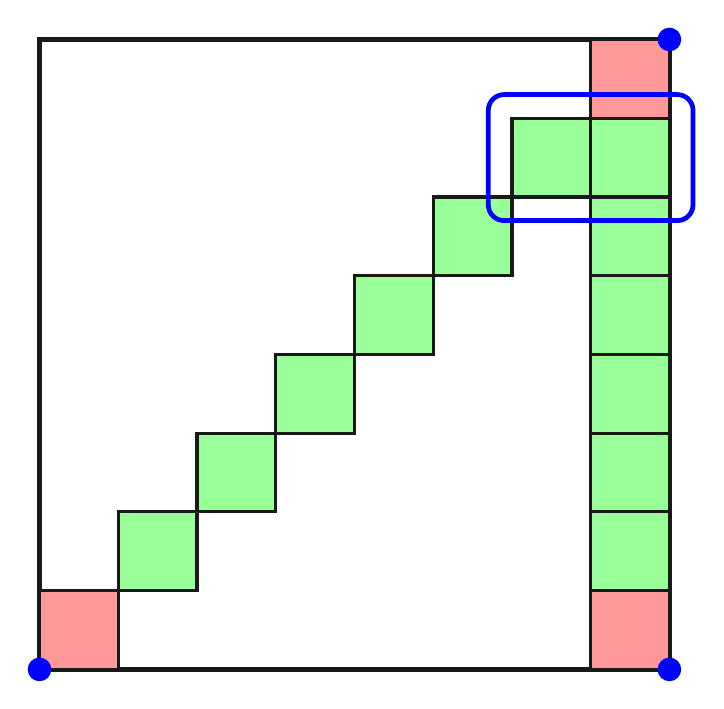
\begin{tikzpicture}
    % \draw[help lines] (0,0) grid (15,3);
    \foreach \x in
        {(0,0)} 
        {\draw[black!90, line width=0.6mm] \x rectangle+(8,8);}
    \foreach \x in
        {(0,0), (7,0),(7,7)} 
        {\draw[redsq] \x rectangle+(1,1);}
    \foreach \x in
        {(1,1), (2,2), (3,3), (4,4), (5,5), (6,6), 
         (7,1), (7,2), (7,3), (7,4), (7,5), (7,6)} 
        {\draw[greensq] \x rectangle+(1,1);}
    \foreach \x in
        {(0,0), (8,0), (8,8)}
        {\fill[blue, ] (\x circle (1.5mm);}
    \draw[blue, line width=0.6mm, rounded corners=2mm] (5.7,5.7) rectangle (8.3,7.3);
\end{tikzpicture}
\end{document}